% Claim:
%   OpenRath scales from one agent to multi-agent workflows by preserving a
%   single runtime value: every stage accepts and returns Session.
% Evidence:
%   /Users/kk/Project/OpenRath/src/rath/flow/agent.py;
%   /Users/kk/Project/OpenRath/src/rath/flow/workflow.py;
%   /Users/kk/Project/OpenRath/src/rath/flow/compressor.py;
%   engineering and research workflow examples.
% Open questions:
%   Future releases should specify parallel scheduling, merge policy, and
%   conflict handling for larger workflow graphs.

Multi-agent design in OpenRath is intentionally small: an agent is a reusable layer, a workflow
is a reusable composition, and the moving runtime value is still Session. This avoids a common
failure mode in agent systems, where a single-agent API works cleanly but the multi-agent version
introduces a new shared mutable object, a hidden message bus, or a controller-only trace.


The engineering examples use this shape for lead-engineer, specialist, and QA roles; the research
examples use the same shape for literature, reproduction, compression, and output stages. The
domain-specific roles differ, but the runtime contract does not. This is the point of the design: a
workflow can grow from a script into a nested agent team without replacing the object that carries
evidence, placement, lineage, usage, and replay state.


This report therefore treats multi-agent capability as a runtime-state claim, not as a claim that
every workflow is already a measured benchmark result. Current evidence verifies deterministic
lineage export, local sandbox packets, workflow transcripts, focused tests, and layout review. Larger
claims about parallel branch scheduling, merge quality, memory quality, and task-level leaderboards remain scoped to follow-on evaluation.

\begin{figure}[!htbp]
\centering
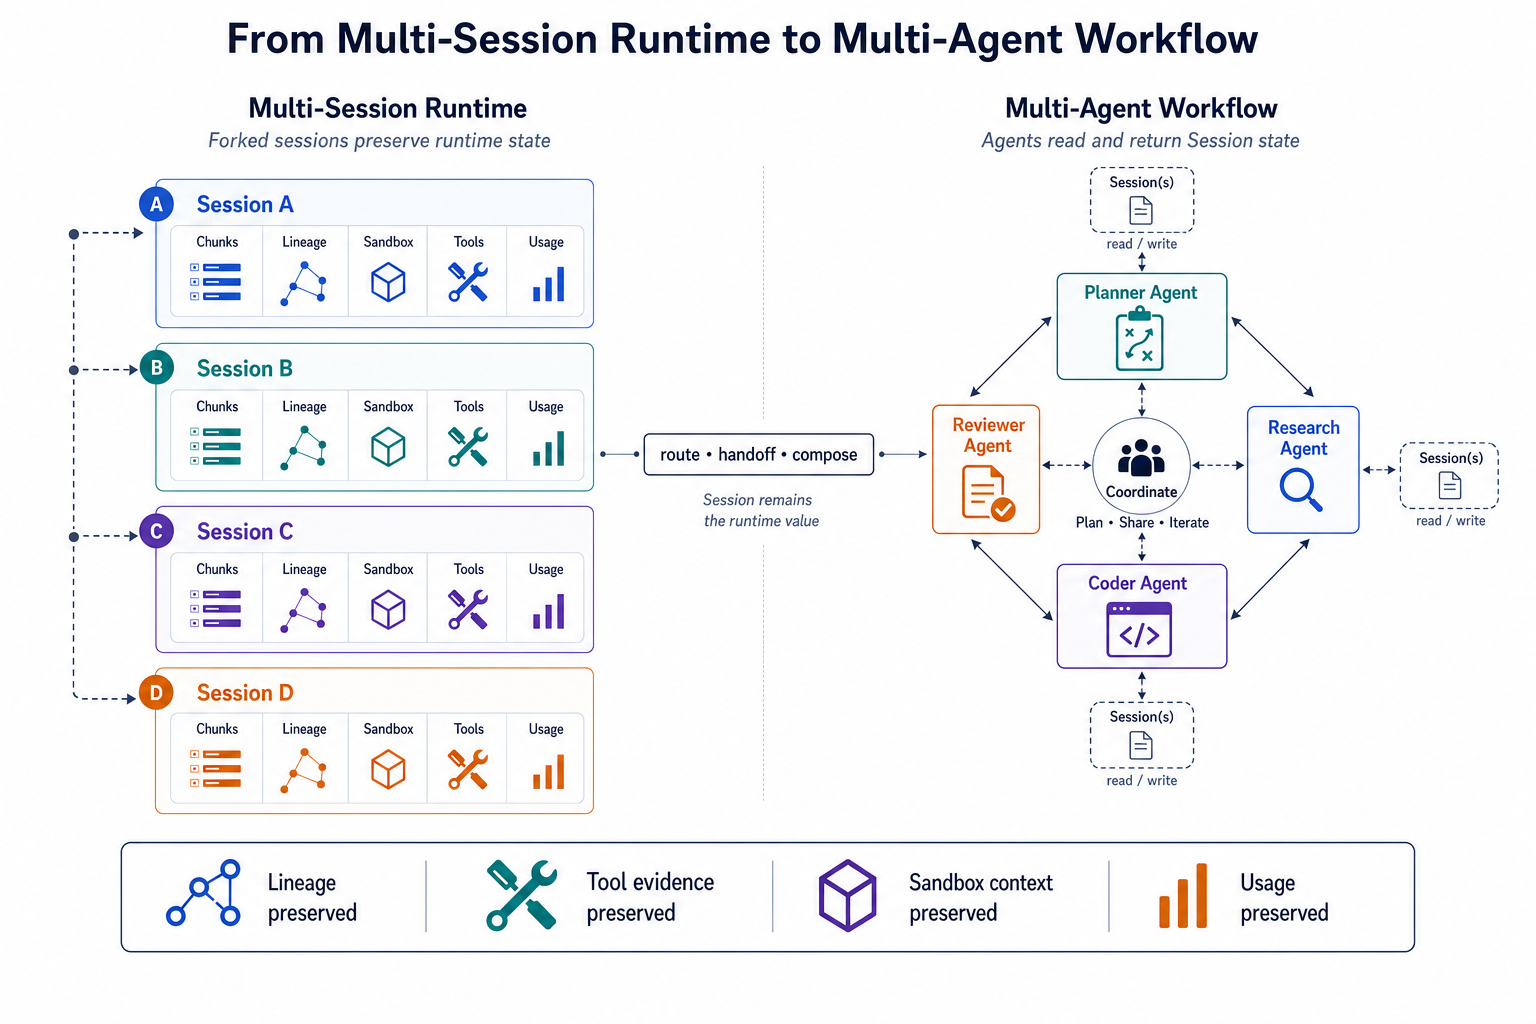
\includegraphics[width=0.98\linewidth]{assets/mermaid-diagrams/multi-session-to-agent-workflow-image2.png}
\caption{Multi-session runtime and multi-agent workflow share the same boundary:
agents route, hand off, and compose work by reading and returning
\texttt{Session} state rather than introducing a second runtime object.}
\label{fig:multi-session-to-agent-workflow}
\end{figure}

\begin{table}[!htbp]
\vspace{0.1em}
\centering
\small
\caption{Multi-agent composition without introducing a second runtime state.}
\label{tab:compact-multi-agent-design}
\begin{tabularx}{\linewidth}{@{}>{\raggedright\arraybackslash}p{0.22\linewidth}>{\raggedright\arraybackslash}X>{\raggedright\arraybackslash}X@{}}
\toprule
Pattern & How it composes & What stays inspectable \\
\midrule
One agent, many sessions & The same agent parameters are applied to fresh, forked, resumed, or sandbox-bound sessions. & Prompt layer stays stable while conversation, placement, lineage, and usage live on the session. \\
Many agents, one state & Specialist agents each consume and return \texttt{Session}; workflows pass the returned value forward. & Intermediate state can be inspected after planning, tool use, compression, QA, or final synthesis. \\
Nested workflows & A child workflow hides internal agent structure behind \texttt{forward(session)}. & Parent workflows see one returned session instead of a private orchestration format. \\
Control surfaces & Chunks, tool results, lineage fields, usage counters, persistence files, and callbacks remain tied to the session. & Failures, budget crossings, branch provenance, and interrupted runs become reviewable artifacts. \\
\bottomrule
\end{tabularx}
\vspace{0.1em}
\end{table}
